\chapter{Mockups}
\label{a:prototipos}

\section{Interfaces do utilizador}
\label{interfaces}

\subsection{Autenticação}

Quando se acede à página oficial da aplicação, é possível ver a descrição do produto, funcionalidades, planos entre outros. É também a partir da página do produto que o utilizador consegue realizar a autenticação na plataforma.

Representado nas Figuras \ref{10q-login} e \ref{10q-registo} temos as interfaces que dizem respeito à autenticação do utilizador.

Quando se efectua o \textit{login} na plataforma, o utilizador é apresentado com a interface representada na Figura \ref{10q-login}, onde é necessário introduzir o email e password associados à sua conta. Caso as credenciais não estejam corretas, o utilizador é notificado para esse efeito.



\begin{figure}[ht!]
	\begin{center}
		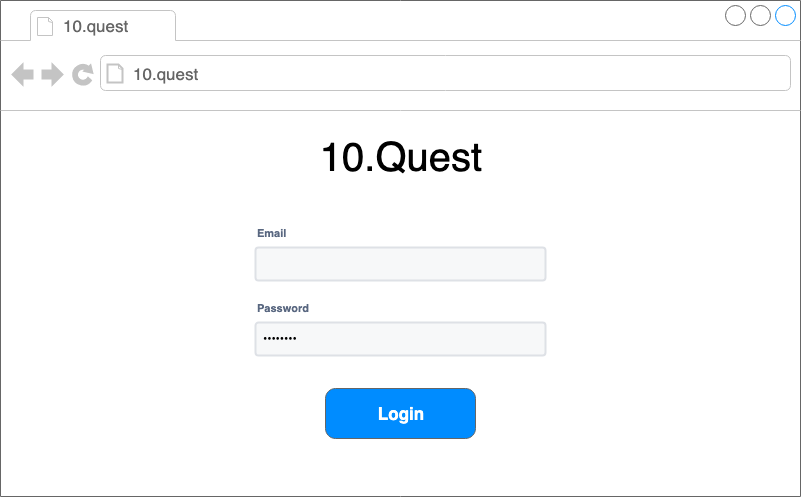
\includegraphics[width=1\textwidth]{img/prototipos/1.png}
		\caption{10.quest - Login}
		\label{10q-login}
	\end{center}
\end{figure}


Para criar uma conta nova, é necessário aceder à pagina de registo da plataforma. Como podemos ver na Figura \ref{10q-registo}  para criar uma conta nove é necessário introduzir o nome, nome da empresa, email, nome de utilizador e password.

\begin{figure}[ht!]
	\begin{center}
		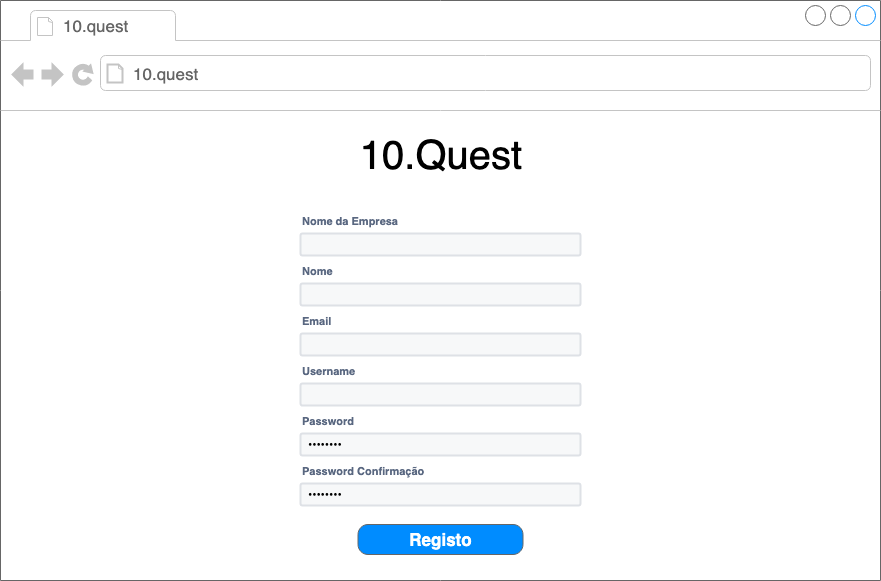
\includegraphics[width=1\textwidth]{img/prototipos/2.png}
		\caption{10.quest - Registo}
		\label{10q-registo}
	\end{center}
\end{figure}

\newpage

\subsection{Página Inicial}

Representado na Figura \ref{10q-home} temos a página principal da plataforma. A partir da página inicial um utilizador autenticado tem acesso a todas as funcionalidades principais do sistema representadas na Figura \ref{d:altonivel}, na secção \ref{rf}.

A partir da páginas principal o utilizador têm acesso às formações, questionários e concursos mais recentes (i. e. os ultimos que criou ou editou) e respectivo estado e, no fundo da página, é ainda possível observar algumas estatísticas globais relativas aos mesmos que serão definidas no segundo semestre.

\begin{figure}[ht!]
	\begin{center}
		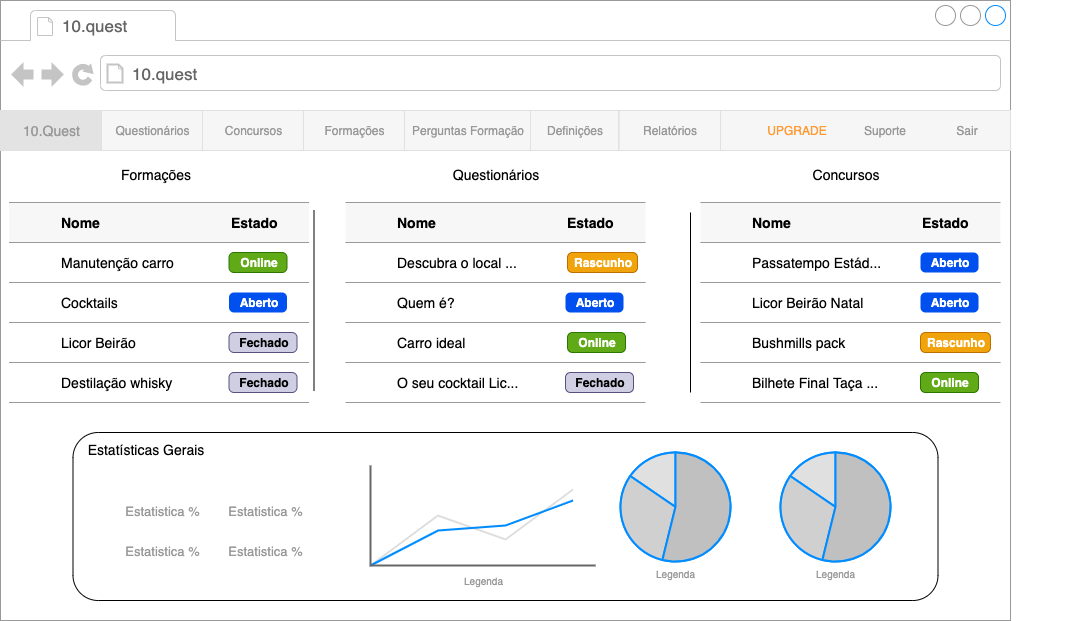
\includegraphics[width=1\textwidth]{img/prototipos/home.png}
		\caption{10.quest - Página Inicial}
		\label{10q-home}
	\end{center}
\end{figure}
\newpage

\subsection{Questionários}

Na Figura  \ref{10q-listaQ} temos página principal dos questionários. Nesta página estão listados todos os questionários associados à conta do utilizador. Para cada questionário é possível ver a data de inicio, data de fim, o estado actual do questionário e ainda alguns dados estatísticos que irão ser definidos no segundo semestre.
Para  apagar um ou mais questionários o utilizador tem que marcar cada um deles e depois carregar no botão para eliminar os questionários. É ainda possível pesquisar um questionário por nome.

\begin{figure}[ht!]
	\begin{center}
		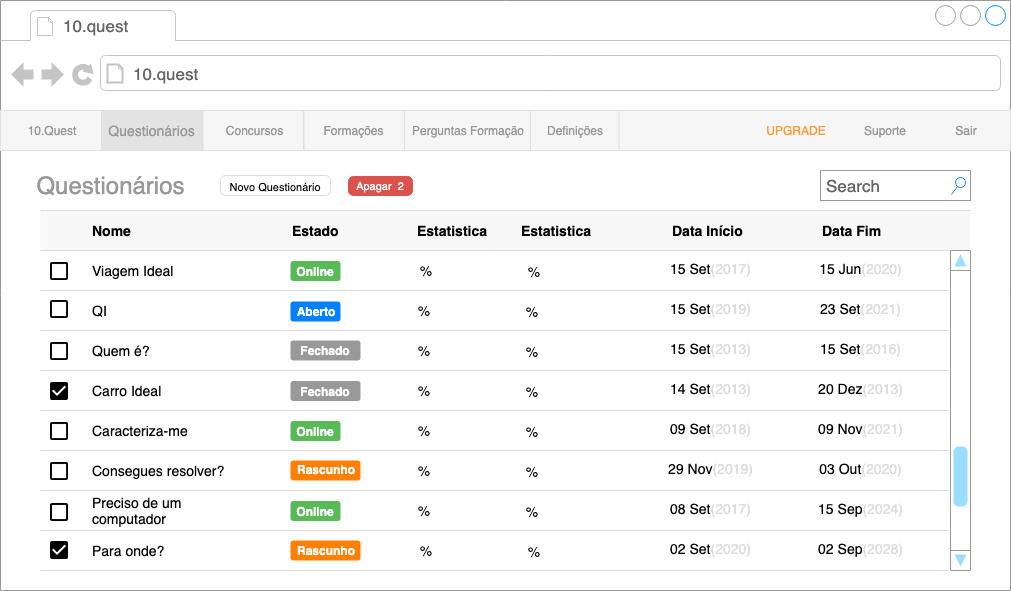
\includegraphics[width=1\textwidth]{img/prototipos/4.png}
		\caption{10.quest - Lista de Questionários }
		\label{10q-listaQ}
	\end{center}
\end{figure}


Para criar um novo questionário, o utilizador carrega no botão para criar um novo questionário e é redirecionado para a página de criação do mesmo, representado na Figura \ref{10q-questoes}.

Numa primeira instância o utilizador tem de criar um conjunto de questões que serão utilizadas para criar o querstionário. Na Figura \ref{10q-Nquestao} podemos observar a criação de uma nova questão.

\clearpage


\mbox{}
\begin{figure}[ht!]
	\begin{center}
		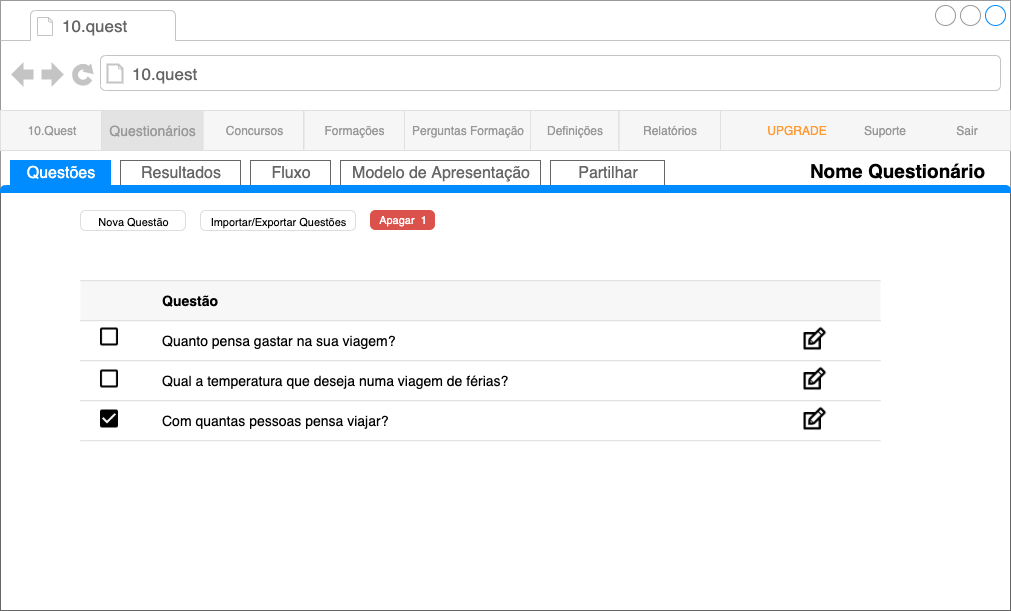
\includegraphics[width=1\textwidth]{img/prototipos/13.png}
		\caption{10.quest - Criar Questionário (Lista de questões)}
		\label{10q-questoes}
	\end{center}
\end{figure}

\begin{figure}[ht!]
	\begin{center}
		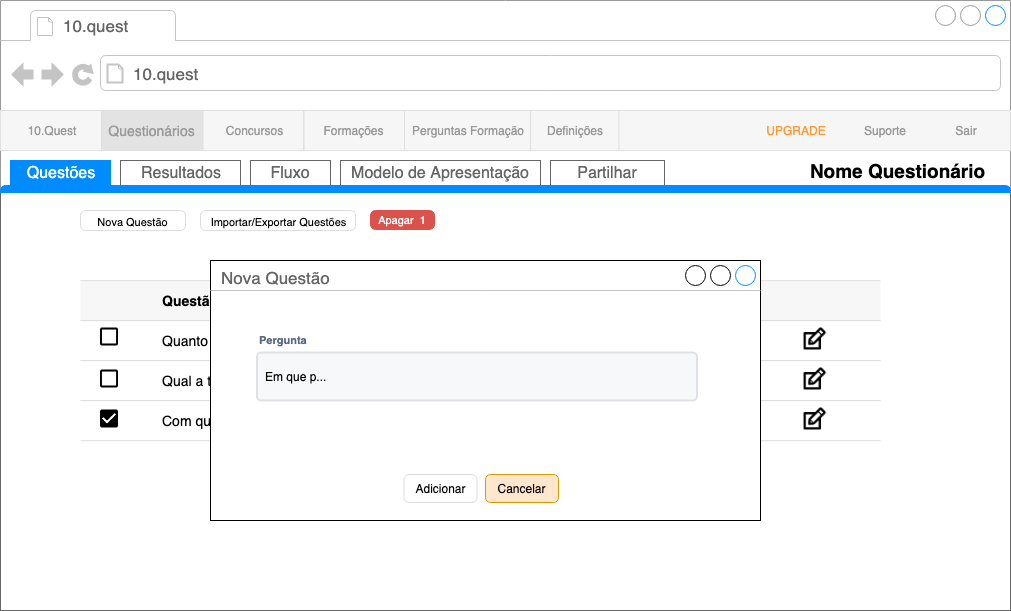
\includegraphics[width=1\textwidth]{img/prototipos/14.png}
		\caption{10.quest - Criar Questionário (Nova Questão) }
		\label{10q-Nquestao}
	\end{center}
\end{figure}
\newpage

Representado na Figura \ref{10q-result} temos a lista de resultados possíveis do questionário. Depois de terminada a criação de todas as questões pretendidas para a criação do questionário, o utilizador segue para a criação dos resultados possíveis para o questionário. 
Representado na Figura \ref{10q-Nresult} temos a criação de um novo resultado. Para criar um novo resutaldo o utilizador necessita de introduzir obrigatóriamente um título e uma tag. O utilizador pode também, opcionalmente, associar um link e/ou um ficheiro de imagem, audio ou vídeo.

\begin{figure}[ht!]
	\begin{center}
		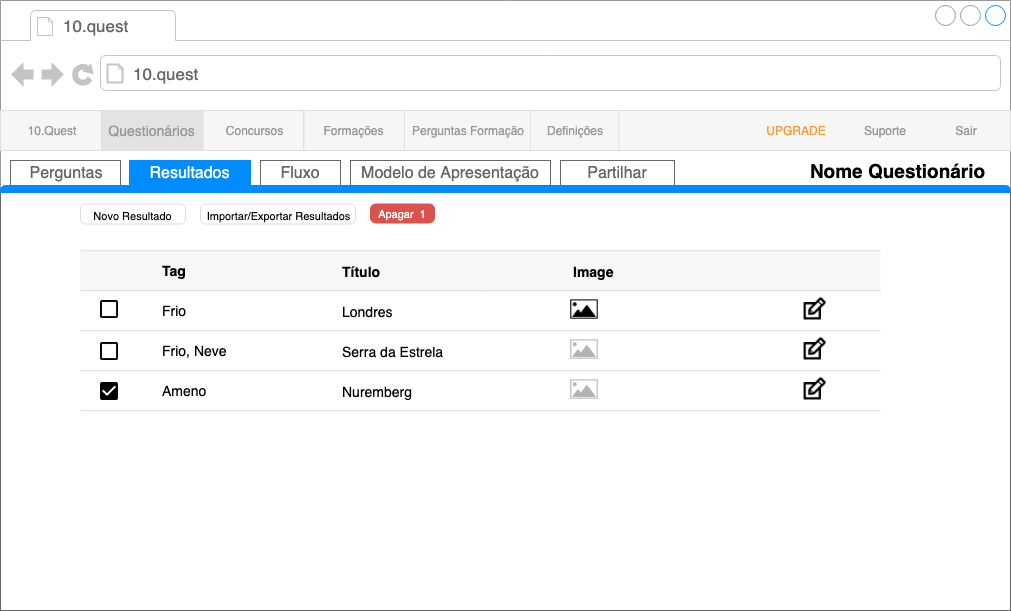
\includegraphics[width=1\textwidth]{img/prototipos/15.png}
		\caption{10.quest - Criar Questionário (Lista de Resultados)}
		\label{10q-result}
	\end{center}
\end{figure}

\begin{figure}[ht!]
	\begin{center}
		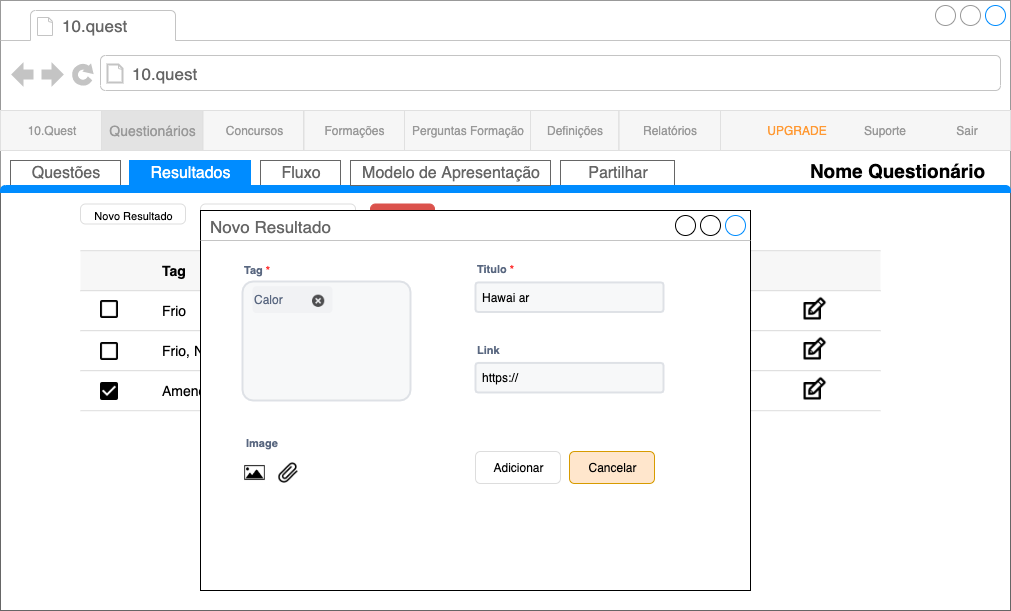
\includegraphics[width=1\textwidth]{img/prototipos/16.png}
		\caption{10.quest - Criar Questionário (Novo Resultado)}
		\label{10q-Nresult}
	\end{center}
\end{figure}
\newpage

Assim que o utilizador adicionar todas as questões e resultados desejados para a criação do questionário, encontram-se as condições necessárias para começar a criar o fluxo lógico. 

Na Figura \ref{10q-fluxo} está representada a página da criação do fluxo lógico do questionário. O utilizador, em primeiro lugar, tem de escolher a pergunta pelo qual quer iniciar o questionário e posteriormente tem de adicionar pelo menos duas respostas. Para cada resposta o utilizador pode adicionar uma ou mais tags (tags que associam os resultados à resposta), e a pergunta que se segue caso a mesma seja escolhida. O peso atribuido a cada pergunta por definição terá o valor de 10, contudo este valor pode ser alterado pelo utilizador

É ainda de notar que a qualquer momento, o utilizador pode voltar atrás e adicionar mais questões e resultados, sendo que o processo do fluxo lógico não é perdido.

\begin{figure}[ht!]
	\begin{center}
		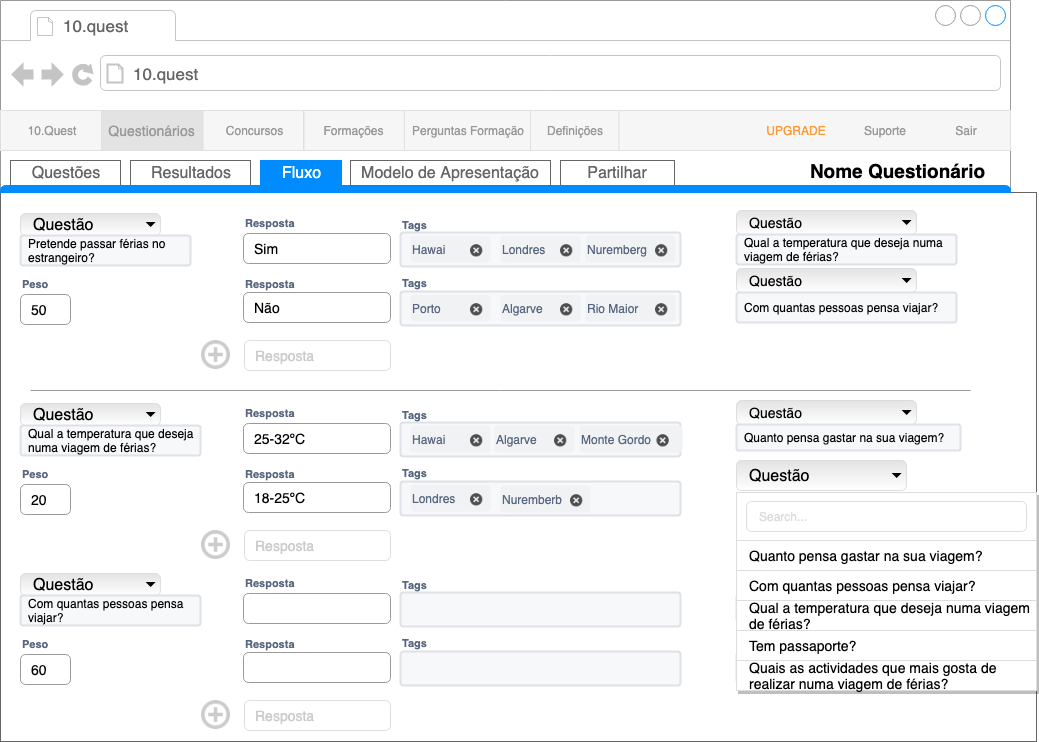
\includegraphics[width=1\textwidth]{img/prototipos/17.png}
		\caption{10.quest - Criar Questionário (Fluxo de questões)}
		\label{10q-fluxo}
	\end{center}
\end{figure}

\newpage


\subsection{Concursos}

Representado na Figura \ref{10q-concursos} temos a página principal dos concursos. À semelhança da secção dos questionários, nesta página estão listados todos os concursos associados à conta do utilizador. Para cada concurso é possível ver a data de inicio, data de fim, o estado actual do questionário e ainda alguns dados estatísticos que irão ser definidos no segundo semestre.
Para  apagar um ou mais concursos o utilizador tem que marcar cada um deles e depois carregar no botão para eliminar os questionários. É ainda possível pesquisar um questionário por nome.

\begin{figure}[ht!]
	\begin{center}
		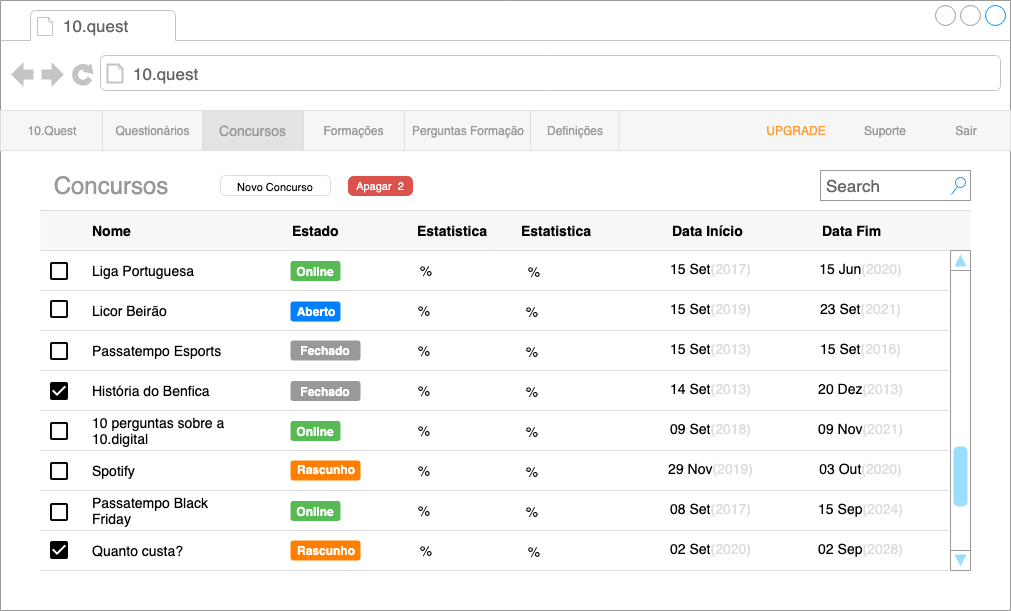
\includegraphics[width=1\textwidth]{img/prototipos/5.png}
		\caption{10.quest - Lista de Concursos}
		\label{10q-concursos}
	\end{center}
\end{figure}

Para criar um novo concurso o utilizador carrega no botão para criar um novo concurso e é redirecionado para a página de criação do mesmo, representado na Figura \ref{10q-Cperguntas}.

Numa primeira instância o utilizador tem de criar um conjunto de perguntas que serão utilizadas para criar o concurso. Na Figura \ref{10q-Npergunta} podemos observar a criação de uma nova pergunta em que o utilizador tem de introdzir a pergunta, a resposta certa e pelo menos uma resposta errada. 


\newpage

\mbox{ }
\begin{figure}[ht!]
	\begin{center}
		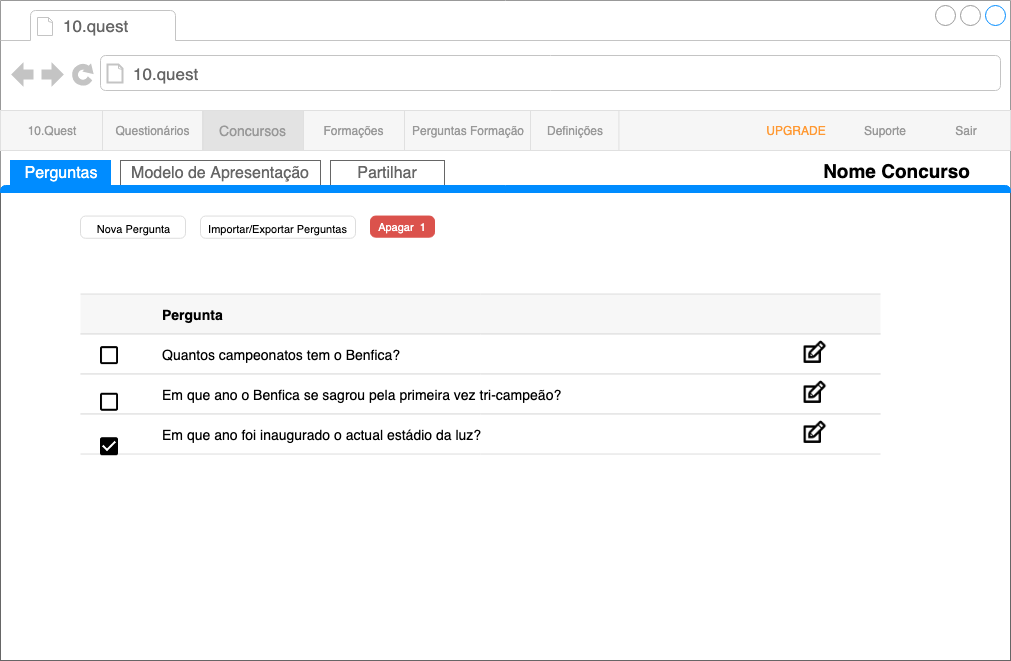
\includegraphics[width=1\textwidth]{img/prototipos/18.png}
		\caption{10.quest - Criar Concurso(Lista de Perguntas)}
		\label{10q-Cperguntas}
	\end{center}
\end{figure}


\begin{figure}[ht!]
	\begin{center}
		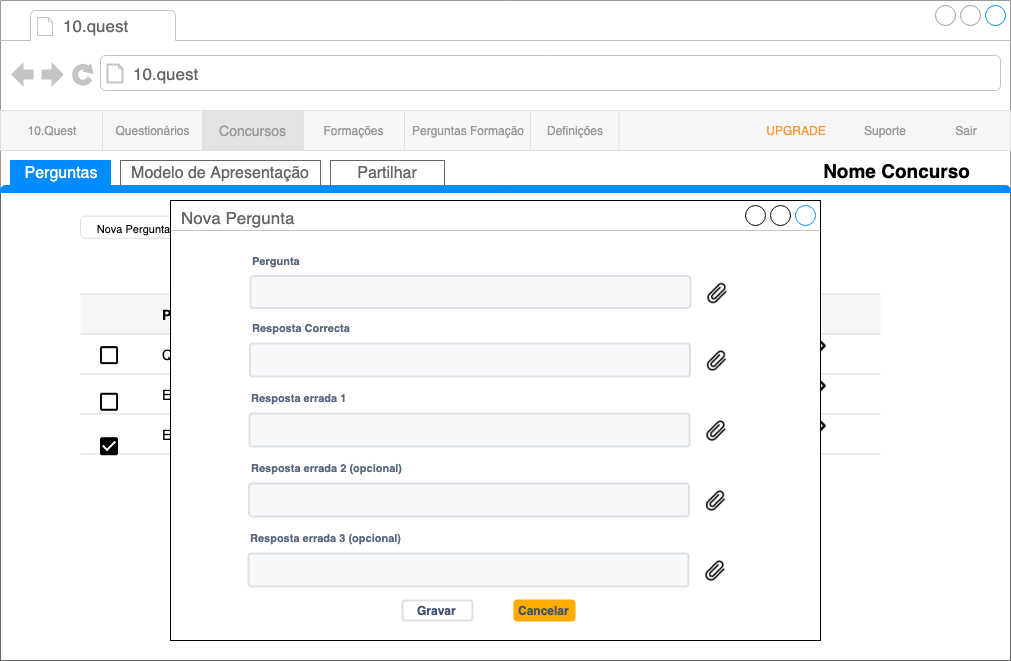
\includegraphics[width=1\textwidth]{img/prototipos/19.png}
		\caption{10.quest - Criar Concurso(Nova Pergunta)}
		\label{10q-Npergunta}
	\end{center}
\end{figure}

\newpage

\subsection{Formações}

Na secção Perguntas Formação temos listadas todas as perguntas de formações, como podemos ver na Figura \ref{10q-perguntasL}. Nesta página o utilizador consegue visualizar, filtrar (por nome ou por tag), eliminar, importar e exportar perguntas. O utilizador consegue ainda criar uma nova pergunta de formação carregando no botão Nova Pergunta.

Representado na Figura \ref{10q-NperguntaF} temos a criação de uma pergunta para uma formação. Como podemos ver, o utilizador tem de obrigatóriamente adicionar uma ou mais tags, a pergunta, uma resposta certa e pelos menos uma resposta errada. O peso associado à pergunta já está pré-definido contudo pode ser alterado pelo utilizador. É ainda possível adicionar uma descrição à pergunta e um ficheiro de aúdio, imagem ou vídeo a uma pergunta e/ou resposta.

\begin{figure}[ht!]
	\begin{center}
		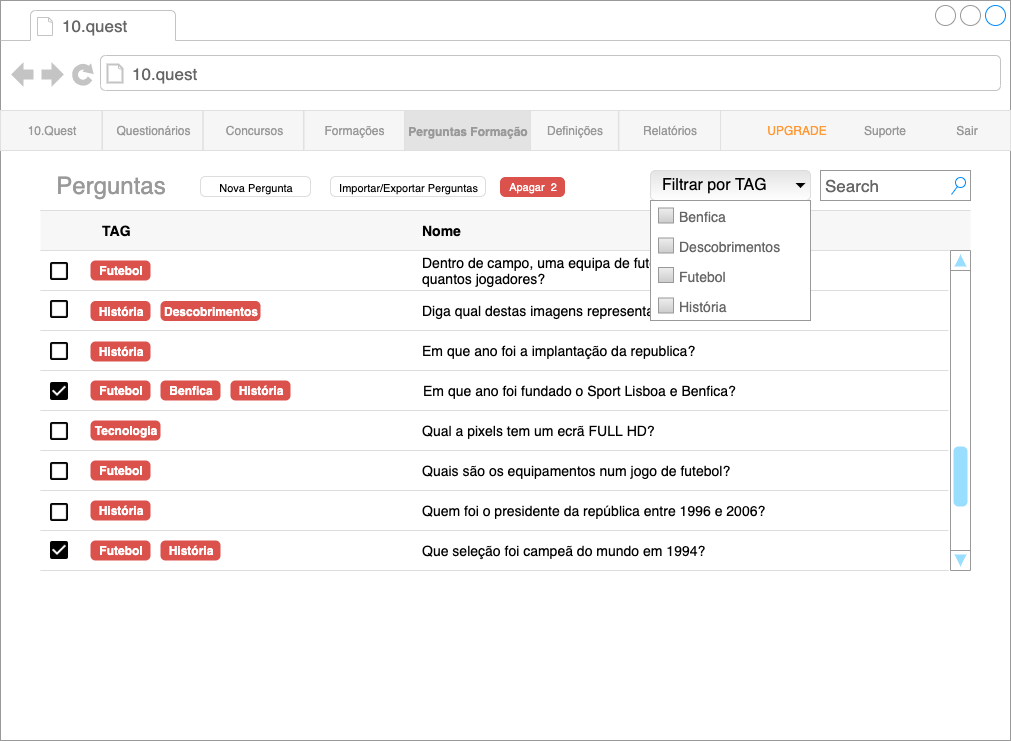
\includegraphics[width=1\textwidth]{img/prototipos/6.png}
		\caption{10.quest - Lista de Perguntas para formação}
		\label{10q-perguntasL}
	\end{center}
\end{figure}

\pagebreak

\begin{figure}[ht!]
	\begin{center}
		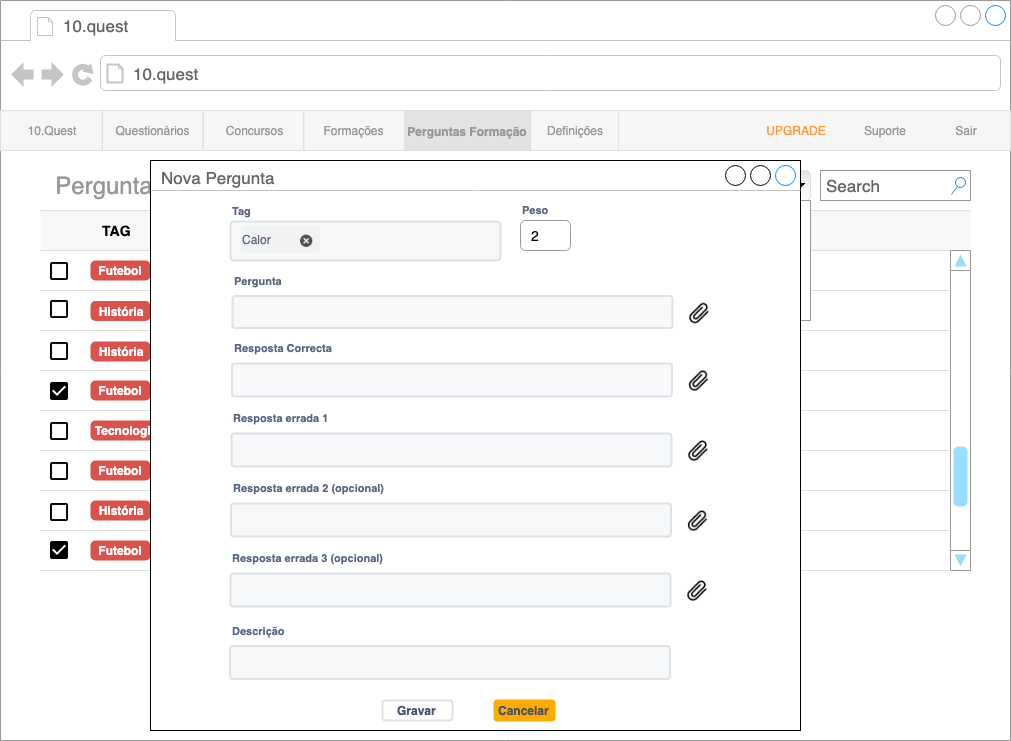
\includegraphics[width=1\textwidth]{img/prototipos/7.png}
		\caption{10.quest - Nova Pergunta para formação}
		\label{10q-NperguntaF}
	\end{center}
\end{figure}


Depois de criadas todas as perguntas necessárias para formação, sendo que o utilizador pode a qualquer momento voltar à página de criação de perguntas para formação e criar novas perguntas, o utilizador está então em condições para criar uma formação.

Representado na Figura \ref{10q-Lformacoes}, temos a secção das formações. Nesta página à semelhança das secções dos questionários e dos concursos, estão listadas todas as formações associadas à conta do utilizador. Para cada formação é possível ver a data de inicio, data de fim, o estado actual do questionário e ainda alguns dados estatísticos que irão ser definidos no segundo semestre.
Para  apagar uma ou mais formações o utilizador tem que marcar cada uma delas e depois carregar no botão para eliminar as formações. É ainda possível pesquisar uma formação por nome.
\newpage

\begin{figure}[ht!]
	\begin{center}
		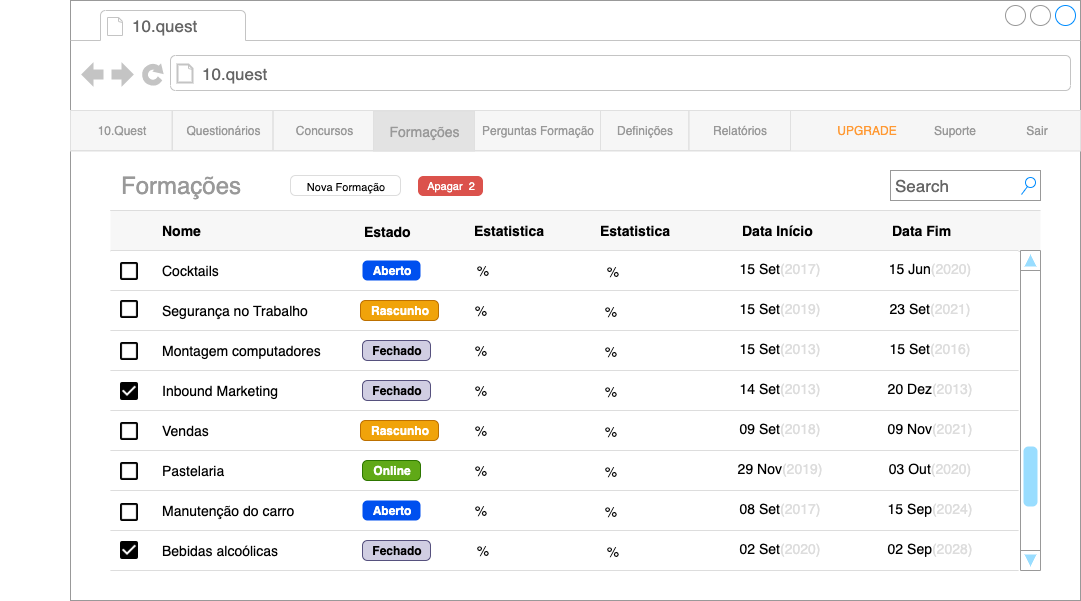
\includegraphics[width=1\textwidth]{img/prototipos/8.png}
		\caption{10.quest - Lista de Formações}
		\label{10q-Lformacoes}
	\end{center}
\end{figure}


Na criação de uma formação o primeiro passo é definir a periocidade do mesmo. Como podemos ver na Figura \ref{10q-periodo}, o utilizador tem introduzir o nome da formação, a data de inicio, a data de fim, os dias da semana em que a notificação da formação será enviada para os utilizadores finais, a hora do envio e a duração/validade da formação. A duração tem de ser menor ou igual ao menor intervalo de tempo possível entre os dias da semana selecionados.

Depois de configurar a periocidade, a formação está criada e o utilizador pode adicionar entradas de perguntas. Representado na Figura \ref{10q-entradas} temos as definições da formação. Nesta página o utilizador pode adicionar e remover uma entrada à formação. Para adicionar uma entrada na formação, o utilizador tem de introduzir a(s) tag(s) de utilizador (i. e. utilizadores finais que estão associados a uma respectiva tag. Os utilizadores finais, quanto se inscrevem numa formação através da landing page, automaticamente ficam associados à(s) tag(s) associadas à formação em questão), a(s) tag(s) de perguntas e o número de perguntas que o utilizador final irá receber daquela entrada.

\newpage

\begin{figure}[ht!]
	\begin{center}
		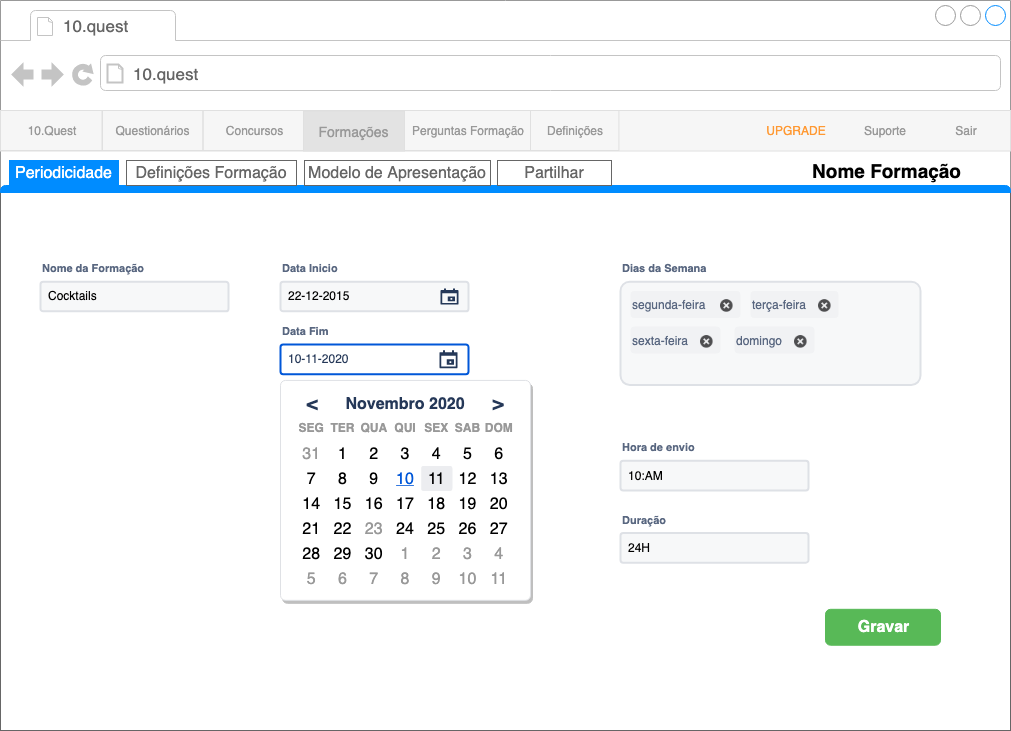
\includegraphics[width=1\textwidth]{img/prototipos/9.png}
		\caption{10.quest - Criar Formação (Periodicidade)}
		\label{10q-periodo}
	\end{center}
\end{figure}

\begin{figure}[ht!]
	\begin{center}
		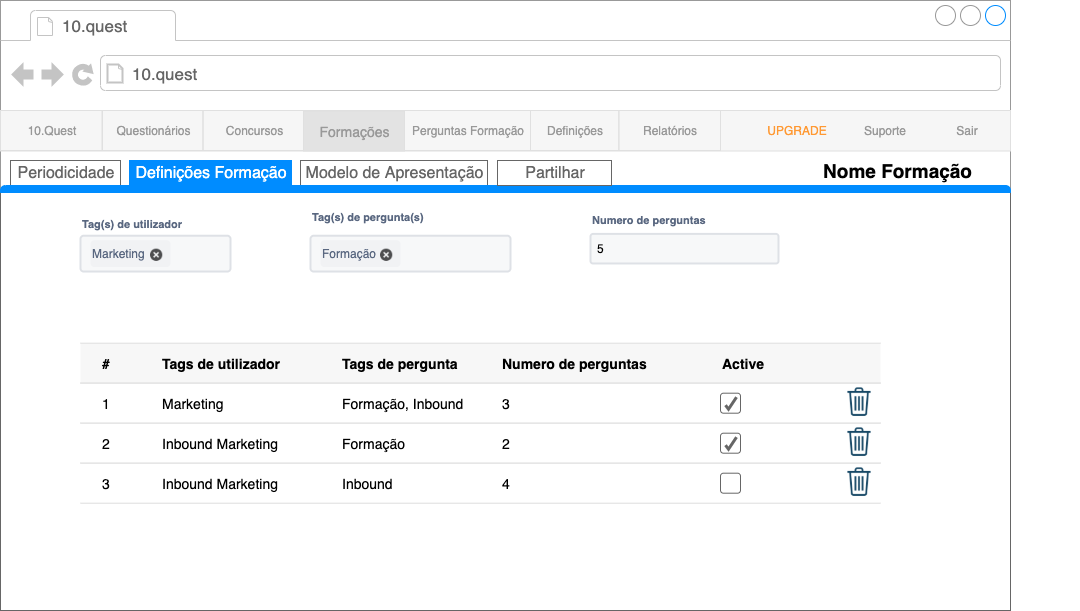
\includegraphics[width=1\textwidth]{img/prototipos/10.png}
		\caption{10.quest - Criar Formação (Definições da Formação)}
		\label{10q-entradas}
	\end{center}
\end{figure}
\newpage

Depois de criada e pré-visualizada a formação (i. e. o utilizador já confirmou que a formação ficou conforme desejado) o utilizador pode personalizar o modelo de apresentação) (Figura \ref{10q-modelo}).

Na secção das notificações por email, o utilizador pode utilizar o \textit{template} do sistema ou utilizar o template alterado. No último o utilizador pode alterar o assunto da formação e personalizar o texto/corpo do email.
Na secção da \textit{landing page} o utilizador tem de inserir o título da página e uma descrição.

Assim o utilizador confirma a publicação da formação, é gerado um link para a \textit{landing page} e estão disponíveis quatro botões para partilhar a formação nas redes sociais.

É ainda de notar que as secções Modelo de Apresentação e Partilhar também se aplicam aos questionários e aos concursos.


\begin{figure}[ht!]
	\begin{center}
		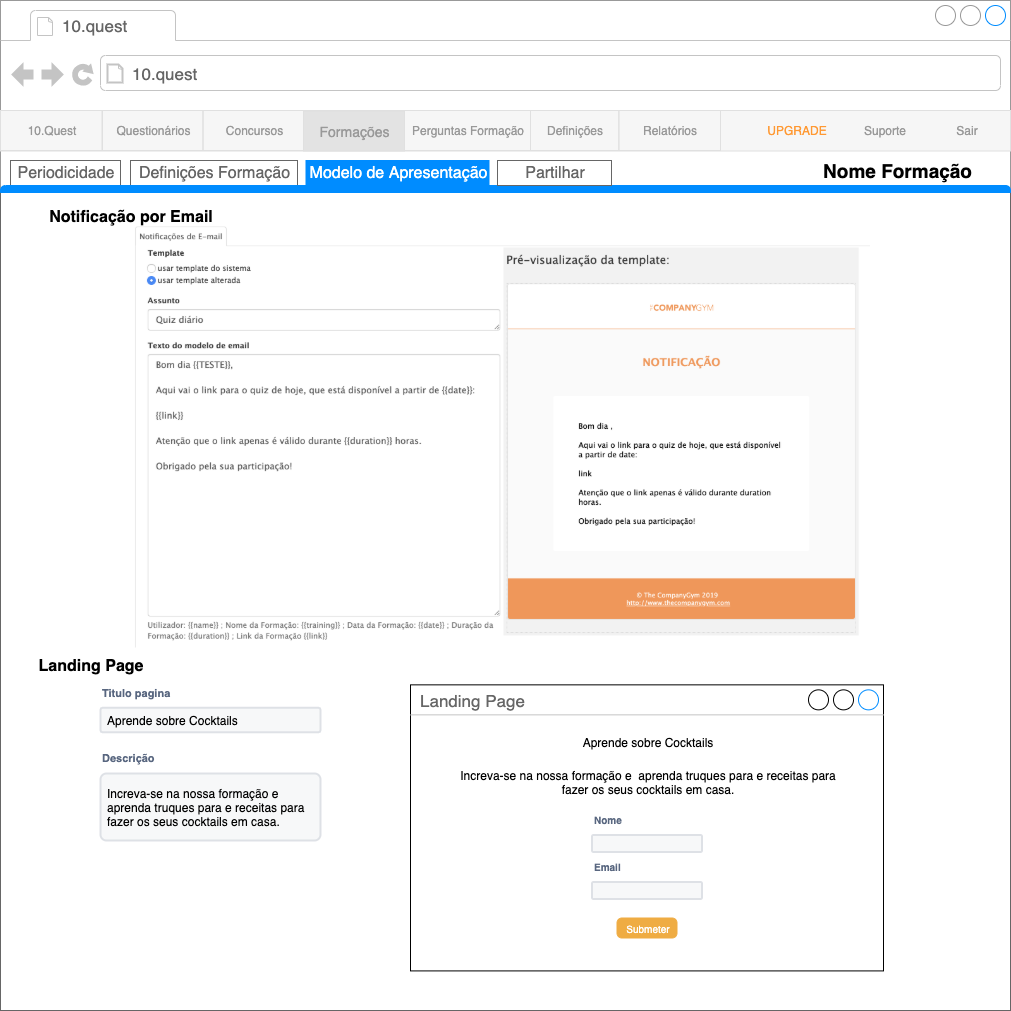
\includegraphics[width=1\textwidth]{img/prototipos/11.png}
		\caption{10.quest - Criar Formação (Modelo de Apresentação)}
		\label{10q-modelo}
	\end{center}
\end{figure}
\clearpage
\mbox{ }

\begin{figure}[ht!]
	\begin{center}
		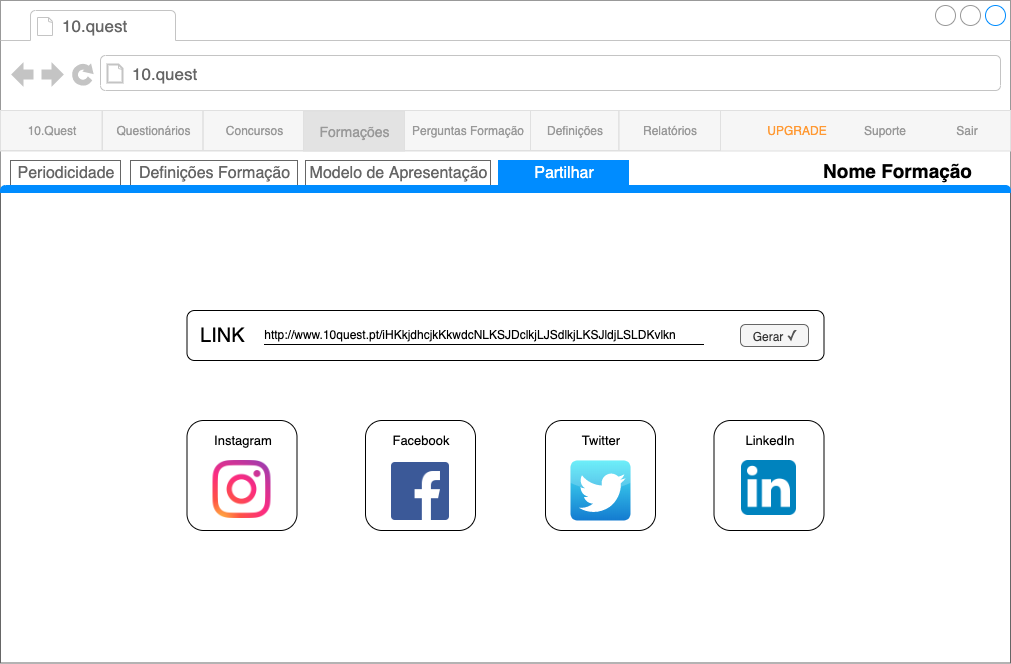
\includegraphics[width=1\textwidth]{img/prototipos/12.png}
		\caption{10.quest - Partilhar Formação}
		\label{10q-}
	\end{center}
\end{figure}


\newpage

\subsection{Relatórios}

A qualquer momento o utilizador pode aceder à página dos resultados gerais das formações, questionários e concursos associados à sua conta. Na página principal dos relatórias, representado na Figura \ref{10q-rel}, o utilizador tem acesso aos resultados gerais, como referido anteriormente, à lista de \textit{leads} e pode também gerar um relatório para uma formação, questionário ou concurso.

Representado nas Figuras \ref{10q-r1}, \ref{10q-r2}, \ref{10q-r3} e \ref{10q-r4}, temos a secção da conversão, perguntas e respostas, resultados e eventos, respectivamente. 

Na conversão o utilizador consegue observar o resultados com maior sucesso e o túnel de conversão. Nas perguntas e respostas o utilizador consegue visualizar todas respostas por pergunta, nos resultados o utilizador consegue ver a quantas pessoas os resultados sairam e dessas pessoas quantas se converteram em leads, e por último, nos eventos o utilizador consegue ver os tipos de eventos (i. e. visualização, participação e submisão) e a conversão (definida na secção da conversão) ao longo do tempo.

\begin{figure}[ht!]
	\begin{center}
		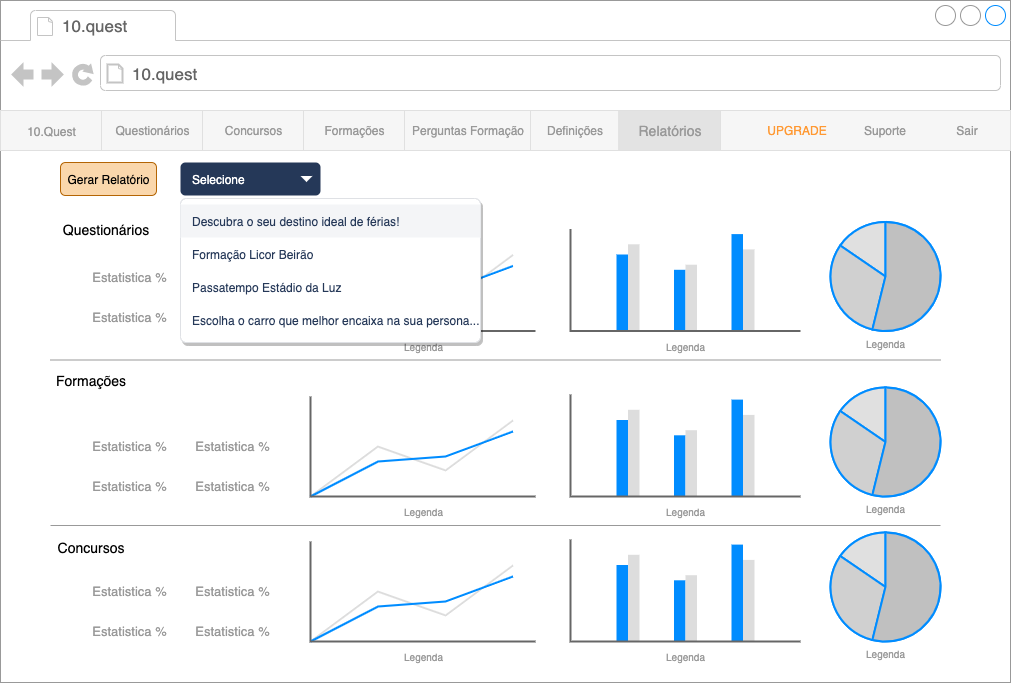
\includegraphics[width=1\textwidth]{img/prototipos/relatorios.png}
		\caption{10.quest - Relatório Geral}
		\label{10q-rel}
	\end{center}
\end{figure}

\begin{figure}[ht!]
	\begin{center}
		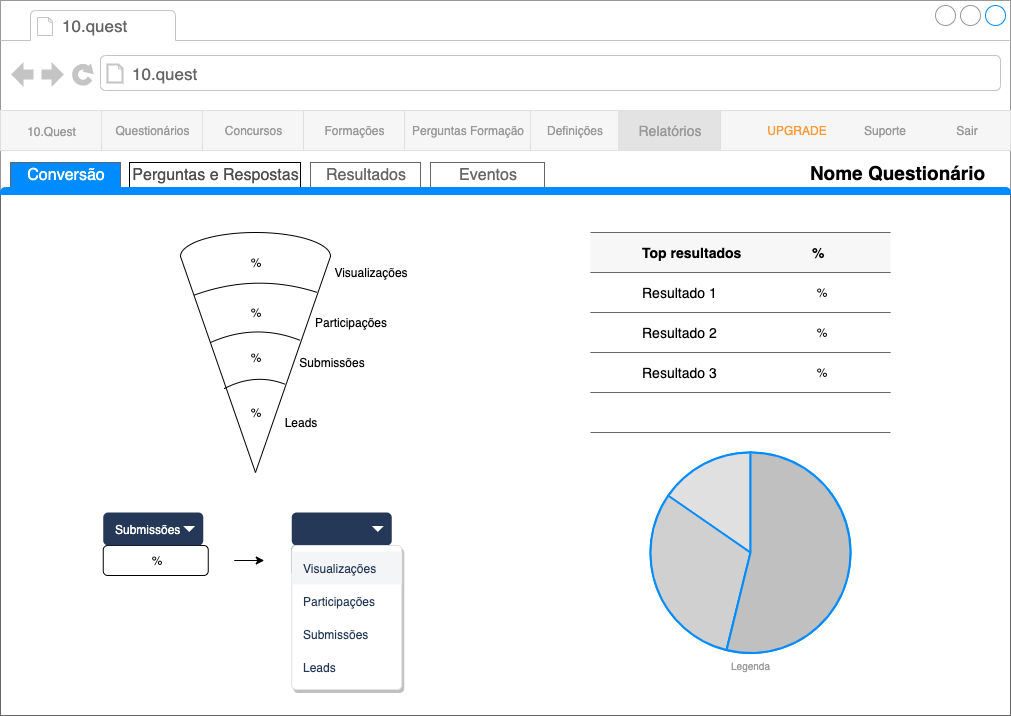
\includegraphics[width=1\textwidth]{img/prototipos/r1.png}
		\caption{10.quest - Relatório Geral}
		\label{10q-r1}
	\end{center}
\end{figure}
\mbox{ }
\newpage
\begin{figure}[ht!]
	\begin{center}
		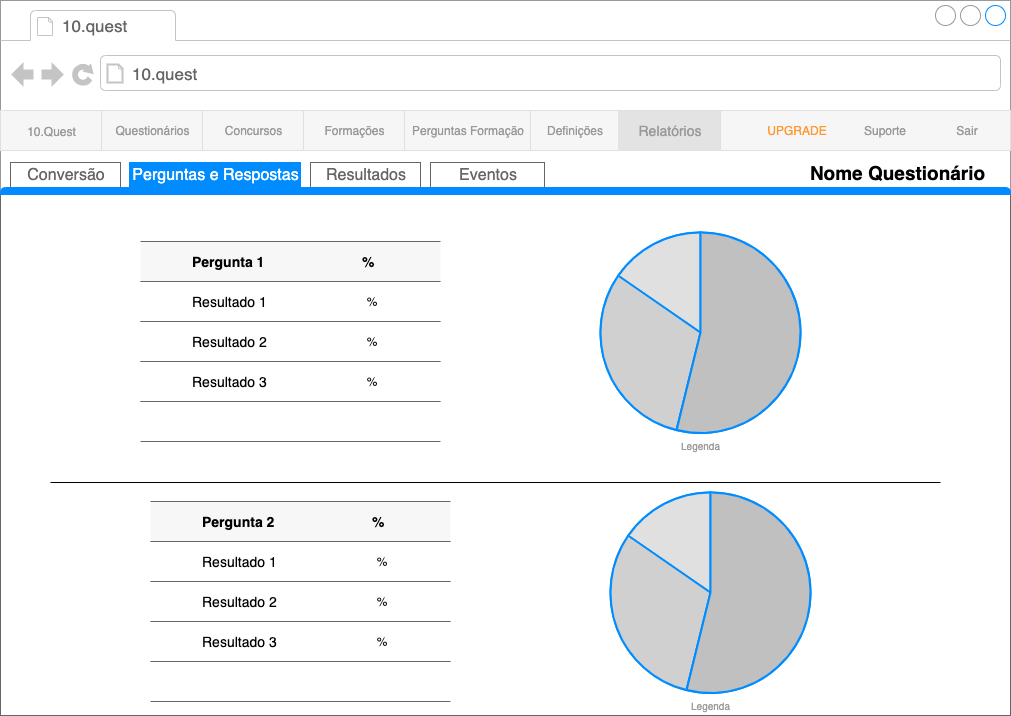
\includegraphics[width=0.95\textwidth]{img/prototipos/r2.png}
		\caption{10.quest - Relatório Geral}
		\label{10q-r2}
	\end{center}
\end{figure}
\newpage
\mbox{ }
\begin{figure}[ht!]
	\begin{center}
		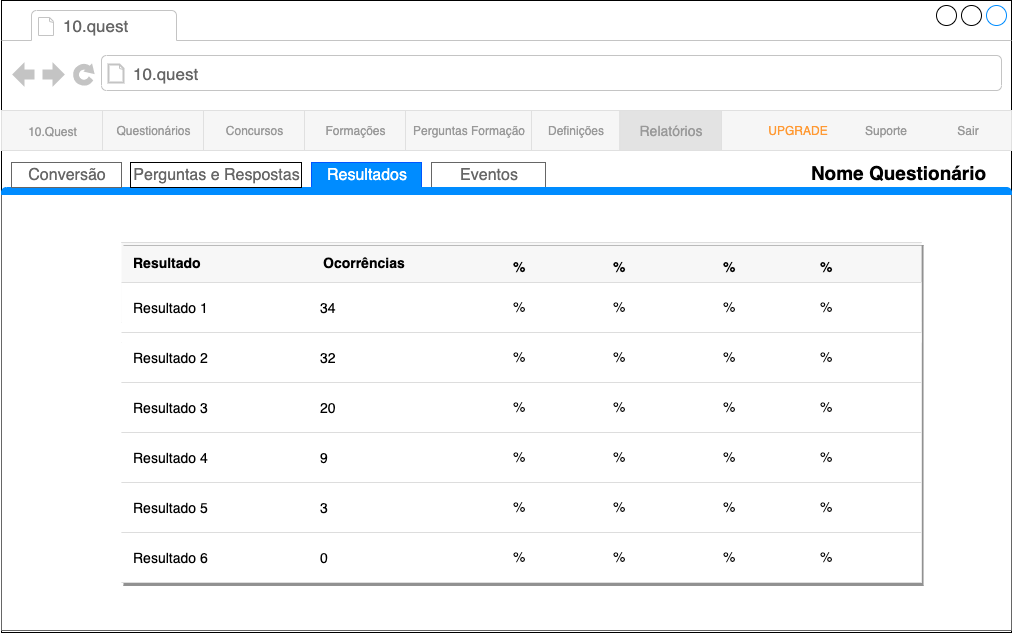
\includegraphics[width=0.95\textwidth]{img/prototipos/r3.png}
		\caption{10.quest - Relatório Geral}
		\label{10q-r3}
	\end{center}
\end{figure}
\mbox{ }
\begin{figure}[ht!]
	\begin{center}
		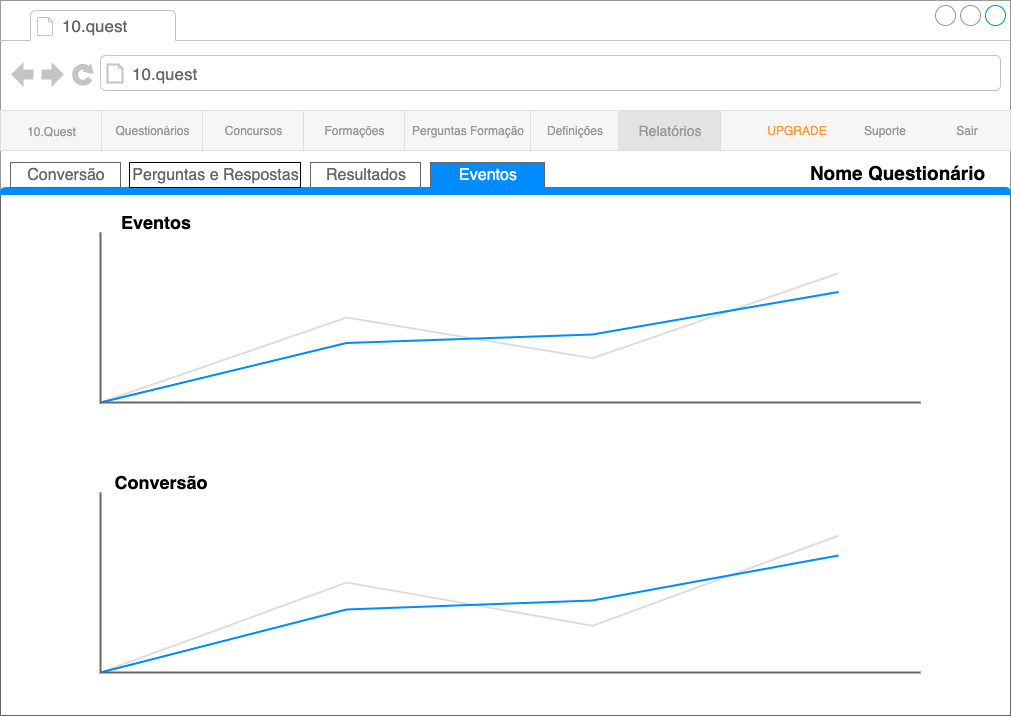
\includegraphics[width=1\textwidth]{img/prototipos/r4.png}
		\caption{10.quest - Relatório Geral}
		\label{10q-r4}
	\end{center}
\end{figure}

\newpage

\begin{figure}[ht!]
	\begin{center}
		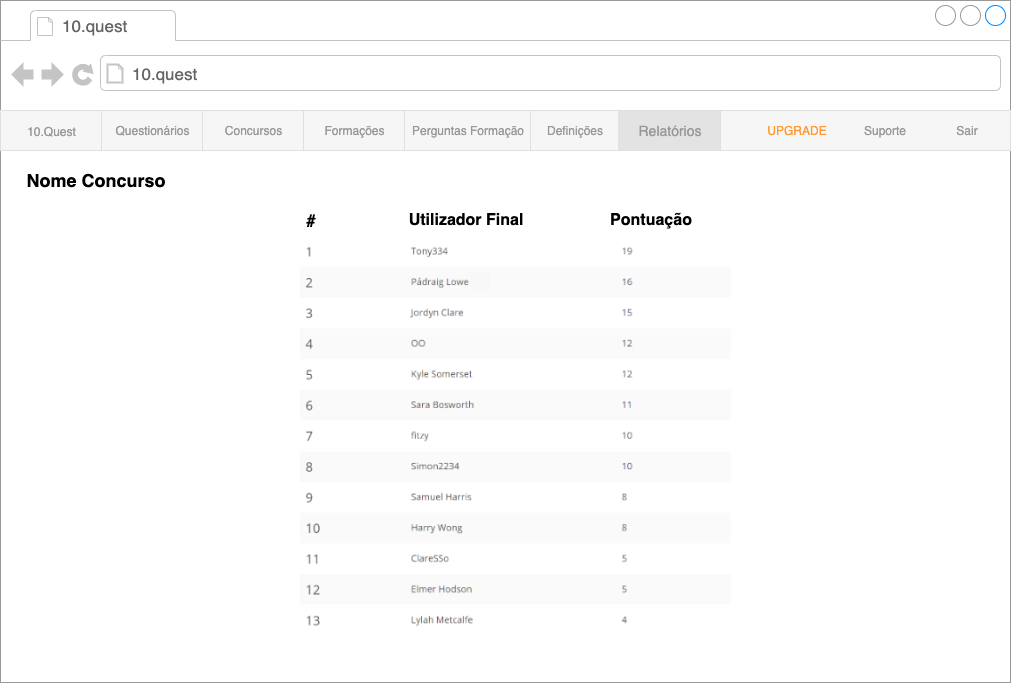
\includegraphics[width=1\textwidth]{img/prototipos/rl.png}
		\caption{10.quest - Relatório Geral}
		\label{10q-t}
	\end{center}
\end{figure}

O utilizador pode também gerar um relatório para um concurso e será aprestentada a tabela de classificações para o respetivo concurso, como podemos ver na Figura \ref{10q-t}

\newpage

\subsection{Definições e Plano de funcionalidades}

Na Figura \ref{10q-def} está representada a páginas das definições da conta de um utilizador. Nesta página o utilizador pode alterar o nome da empresa, email, password e dados de pagamento.

Representado na Figura \ref{10q-plano} temos a página de informações em relação ao plano de pagamento, ou por outras palavras, os pacote de funcionalidades disponíveis para subscrever.

\begin{figure}[ht!]
	\begin{center}
		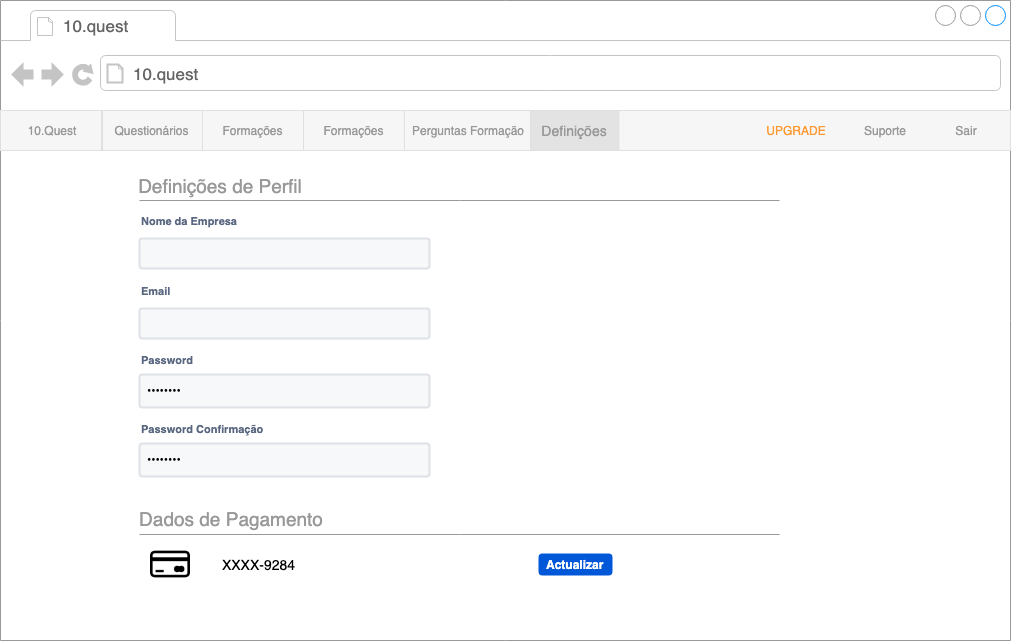
\includegraphics[width=1\textwidth]{img/prototipos/20.png}
		\caption{10.quest - Definições}
		\label{10q-def}
	\end{center}
\end{figure}

\begin{figure}[ht!]
	\begin{center}
		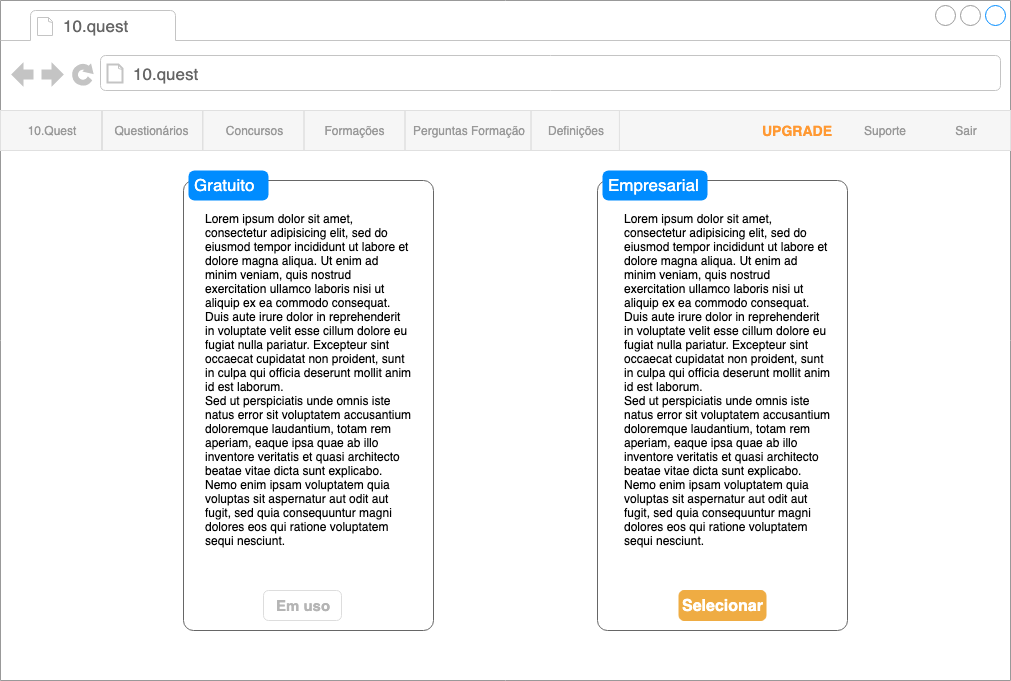
\includegraphics[width=1\textwidth]{img/prototipos/21.png}
		\caption{10.quest - Planos e Preços}
		\label{10q-plano}
	\end{center}
\end{figure}




